\documentclass{article}
\usepackage{amsmath, fullpage}
\usepackage[portuguese]{babel}
\usepackage{graphicx}
\usepackage{color}
\usepackage[normalem]{ulem}
\usepackage{fancyhdr}

\newcommand{\uvec}[1]{\boldsymbol{\hat{\textit{#1}}}}

\pagestyle{fancy}
\fancyhf{} % limpa tudo

% Cabeçalho
\fancyhead[L]{\textbf{Matéria:} TEORIA DE FÍSICA DOS DISPOSITIVOS ELETRÔNICOS\\
\textbf{Professor:} MARCUS VINICIUS BATISTUTA}

\fancyhead[R]{
\includegraphics[width=2.5cm]{unb_logo.png}}

\renewcommand{\headrulewidth}{0.4pt} % linha horizontal
\setlength{\headheight}{10pt} % importante por causa da imagem
\setlength{\headsep}{5pt}    % espaço abaixo do cabeçalho
\begin{document}

\title{Induzindo uma IA ao erro com Fenômenos de Transporte}
\author{Henrique de Oliveira Bernardes - 231011471}

\maketitle

% força o cabeçalho também na primeira página
\thispagestyle{fancy}
\section{Introdução}
Fenômenos de transporte é uma importanta matéria no currículo das engenharias, estudando como massa, calor e quantidade de movimento se transferem em sistemas físicos. Esses processos estão presentes em praticamente todas as áreas da engenharia e da tecnologia, e permite entender as dinâmicas dos escoamentos de fluidos, das trocas de calor e, assim, nos permite projetas sistemas tendo como base estes conhecimentos.

Por outro lado, a inteligência artificial vem tomando cada vez mais destaque em todos os ramos da ciência; isso, contudo, vem com um lado negativo, pois nos faz pensar que ela se tornou detentora de todo conhecimento correto quando, na verdade, ela se baseia em informações alimentadas a ela, sendo essas informações corretas ou erradas.

Assim sendo, esse curto estudo demonstra como uma IA bastante avançada ainda comete erros na resolução de um exercício de fenômenos de transporte.

\section{Metodologia}
\begin{figure}[!h]
  \begin{center}
    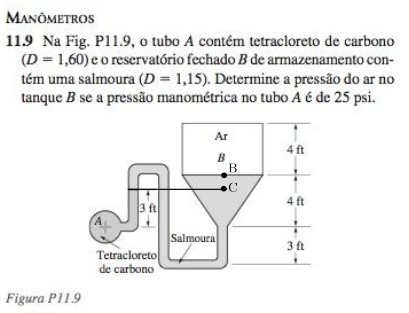
\includegraphics[width=0.35\textwidth]{ExercicioFETRANSAModificado.png}
  \end{center}
  \caption{Exercicio número 11.9 do livro x}\label{fig:}
\end{figure}

O estudo foi feito da forma mais simples: obteve-se um exercício bem conhecido de um livro utilizado na disciplina na própria UnB() e, então, alimentou-se a IA \textit{Gemini} com o enunciado. Finalmente, foi observado o processo de resolução e resultado final, comparando tanto com a resposta desenvolvida no próprio estudo quanto com a resposta disponibilizada pelo solucionário do livo.
\section{Resultados}
Primeiramente, mostramos a forma que a IA \textit{Gemini} propos como solução:
\begin{figure}[!h]
  \centering
  \hfill
  \begin{minipage}{0.35\textwidth}
    \centering
    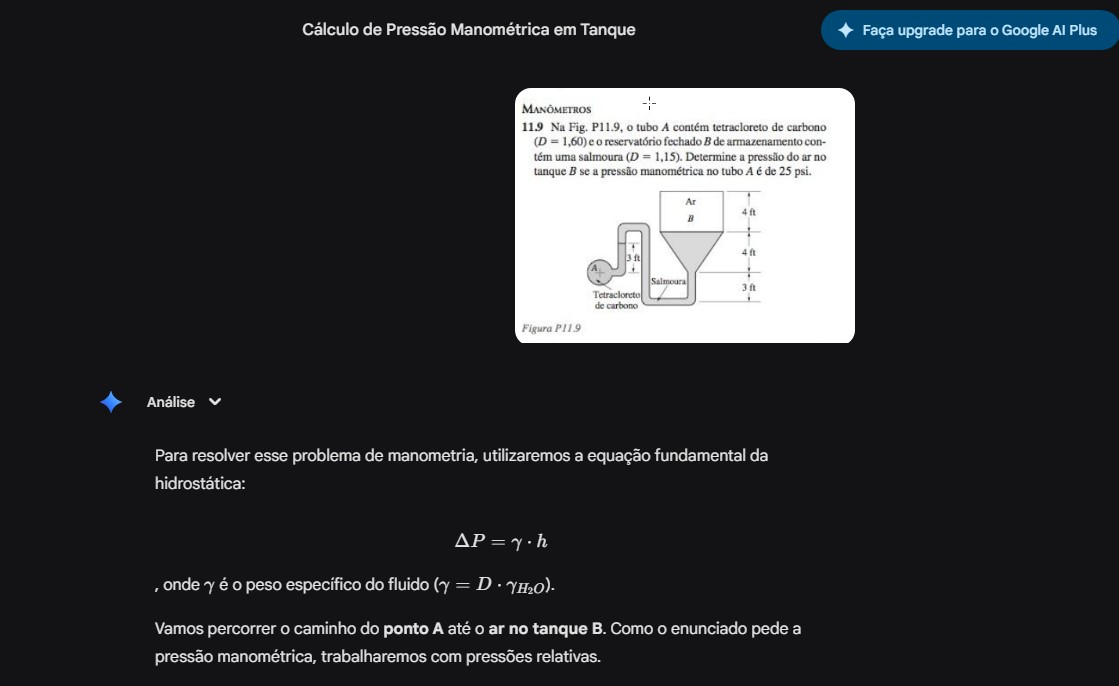
\includegraphics[width=\linewidth]{IA1.jpg}
    \caption{Solução IA 1}
  \end{minipage}\hfill
  \hfill
  \begin{minipage}{0.35\textwidth}
    \centering
    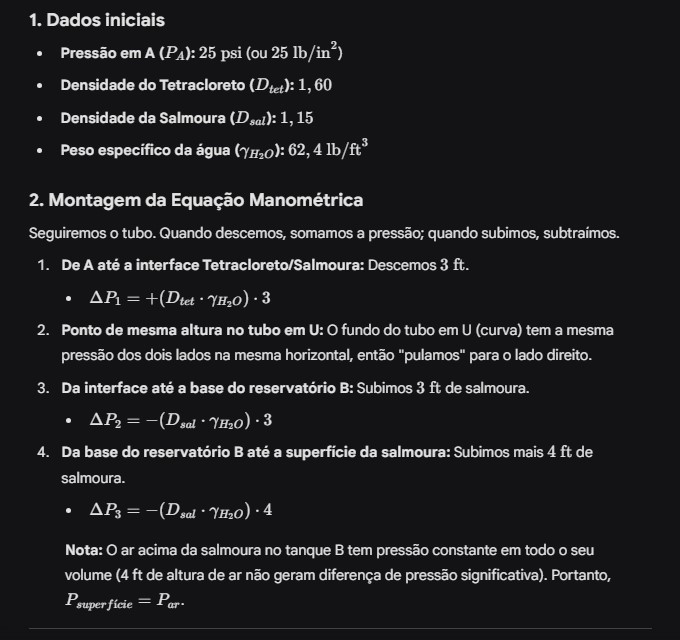
\includegraphics[width=\linewidth]{IA2.jpg}
    \caption{Solução IA 2}
  \end{minipage}
  \hfill
  \begin{minipage}{0.35\textwidth}
    \centering
    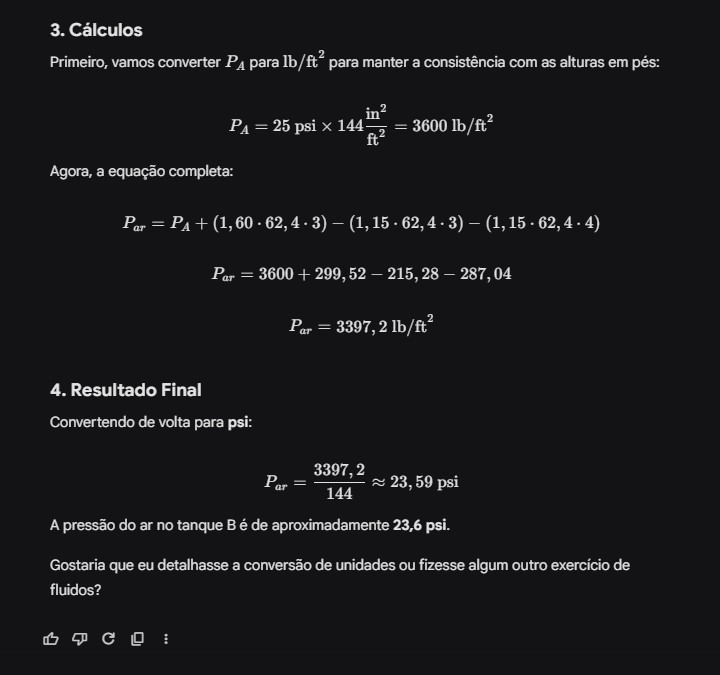
\includegraphics[width=\linewidth]{IA3.jpg}
    \caption{Solução IA 3}
  \end{minipage}
\end{figure}
Pelo solucionário, obtemos a seguinte resolução:

Sabemos que a diferença de pressão entre A e B é:
\begin{align*}
  \gamma_{brine}*h_{BC}+\gamma_{ccl_4}h_{CA}&=p_A - p_B\\
  \gamma_{brine}*(1ft)+\gamma_{ccl_4}(3ft)&=p_A - p_B\\
\end{align*}
Substituindo os valores e isolando a pressão em \(B\), obtemos:
\begin{align*}
  p_B&=\left(25\frac{lbf}{in^2}\right)\left(144 \frac{in^2}{ft^2}\right)-(1.15)\left(62.4 \frac{lbf}{ft^3}\right)(1ft)-(1.60)\left(62.4 \frac{lbf}{ft^3}\right)(3ft)\\
  p_B&=3230 \frac{lbf}{ft^2}\left(\frac{1 ft^2}{144 in^2}\right) = 22.4 psi
\end{align*}
Assim sendo, observamos um erro cometido pela IA ao afirmar que o valor da pressão em B seria \(23.59psi\), ao invés de \(22.4psi\), como comprovado pelos cálculos.
\end{document}
